\section{Introduction}\label{sec:intro}

Modern turbulence modelling has changed its mathematics---from Prandtl's boundary-layer
construction, through Reynolds-averaged and large-eddy simulation, to learned generative
fields---but it keeps reaching the same physical obstacle: the wall
\cite{prandtl1904,pope2000,piomelli2002wall,bose2018wmles}. A geometrically thin near-wall layer
sets skin friction; reversal of wall shear
accompanies separation; and the resulting vorticity, shear layers and wakes organise flow well
beyond it \cite{schlichting2017boundary,pope2000}. Coherent near-wall motions sustain turbulence,
while outer scales partly predict them at high Reynolds number
\cite{robinson1991coherent,jimenez1999autonomous,mathis2009amplitude,marusic2010predictive,smits2011highre,lee2015direct}. Resolving this
small region dominates simulation cost at engineering Reynolds numbers
\cite{chapman1979computational,choi2012grid}; conventional simulation has therefore spent
decades coupling unresolved wall physics to a resolved outer flow
\cite{schumann1975subgrid,cabot2000approximate,larsson2016wmles}. Generative models do not escape
that physics simply by learning the field.

Machine learning now supplies data-driven closures, solver acceleration and learned operators
\cite{ling2016reynolds,duraisamy2019turbulence,kochkov2021machine,brunton2020machine,vinuesa2022enhancing,li2021fno,lu2021deeponet}.
Generative families represent whole-field distributions for inflow, wakes, reconstruction,
super-resolution and subfilter closure
\cite{goodfellow2014gan,ho2020ddpm,song2021sde,karras2022edm,lipman2023flow,
kim2020deep,drygala2022generative,lienen2024zero,buzzicotti2021reconstruction,stengel2020adversarial,bode2021piesrgan,kohl2024benchmarking,dong2025stochclosure},
with conditional variants reconstructing fields from partial observations
\cite{chung2023dps,song2023pigdm,wang2023ddnm,shu2023pidiffusion,rybchuk2023}. Yet two properties
create a wall-specific failure mode: neural networks preferentially fit low-frequency,
large-scale content \cite{rahaman2019spectral,oommen2026learning}, and a volume-averaged loss
weights a thin wall band by cell count rather than by dynamical leverage. A boundary-localised
error can therefore contribute little to a global objective while materially changing drag or
separation (Supplementary Table~13). Validation inherits the same weighting: a volume-averaged
score can certify a reconstruction whose implied wall stress is wrong. Wall treatment is not a
niche refinement of a whole-field
model; it limits what that model can establish wherever surface forces matter.

Representative whole-field formulations are not universally wall-blind: Gao \emph{et al.}
generate wall-bounded fields
\cite{gao2023bayesian}; CoNFiLD includes periodic-hill, rough-wall and channel cases and
documents larger discrepancies near the wall \cite{du2024confild}; Oommen \emph{et al.} address
super-resolution, forecasting and sparse reconstruction
\cite{fukami2019jfm,fukami2021nmi,kim2021unsupervised,oommen2026learning}. Our concern
is not that wall-bounded examples are absent, and we are not claiming that machine learning
universally ignores walls. Yet whole-field objectives do not by
themselves give a thin wall region its engineering weight, and none has an explicit
wall-closure-to-generator interface.

Wall-focused work provides important counterexamples: early neural models of near-wall
turbulence \cite{milano2002neural}, turbulent fields estimated from wall shear and pressure
\cite{guastoni2021convolutional,guemes2021coarse,cuellar2024three}, low-order wall-bounded
surrogates \cite{srinivasan2019predictions,nakamura2021convolutional}, learned synthetic inflow
\cite{wu2017inflow,fukami2019synthetic,kim2020deep}, conditional flow matching from wall
observations \cite{parikh2026conditional} and latent-diffusion wall-pressure reconstruction
\cite{fan2025wallpressure}. In parallel, wall models represent the unresolved near-wall layer for
large-eddy simulation \cite{kawai2012wall,yang2015integral,park2014improved,yang2017llm,bae2019dynamic},
including machine-learning wall models \cite{yang2019predictive,bae2022scientific} extended to
pressure-gradient and separated regimes \cite{lozanoduran2023building,dupuy2023wallmodel}. The
strands answer different questions---which field is compatible with supplied wall data, versus
which unresolved surface quantity can be supplied to a resolved computation---and neither role
substitutes for the other in a coupled simulation.

Two things are missing between them. There is no tested \emph{interface}: no whole-field generative
formulation takes its wall boundary from a closure---generative models have
produced closure terms \cite{dong2025stochclosure}, not consumed a wall model's output---and
no wall closure has been judged by what a generator can propagate from it. And there is no \emph{standard} for testing one---no agreed way
to show that a record can detect wall information at all before it is used to argue that wall
information does or does not matter. Without that, a generative model responding to nothing and a
wall channel carrying nothing produce the same measurement.

\begin{figure}[t]
\centering
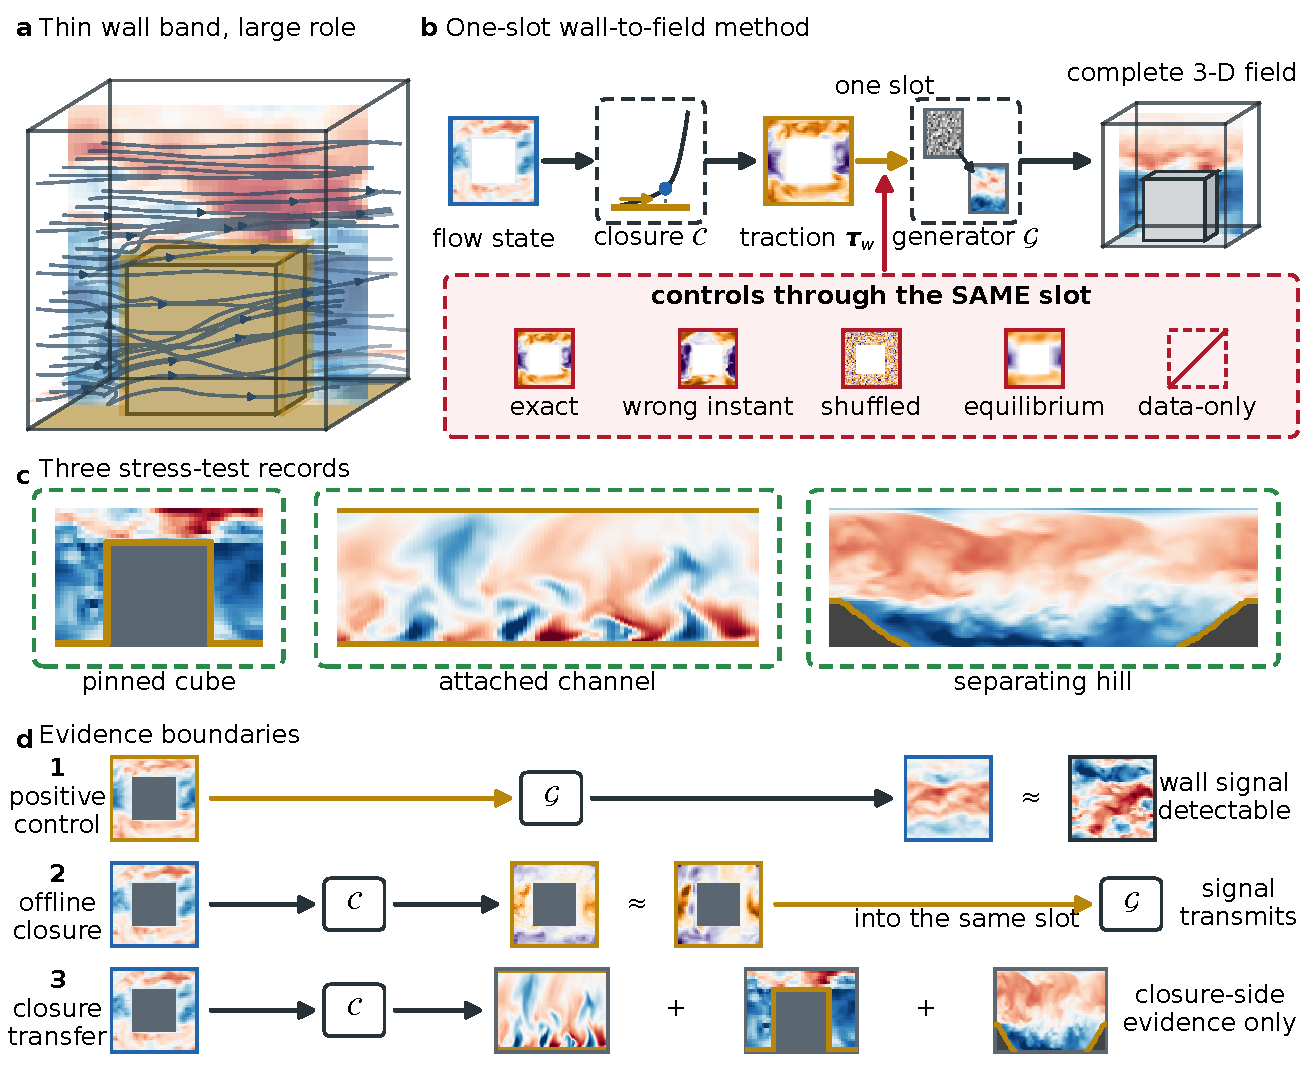
\includegraphics[width=\linewidth]{figures/fig1_architecture.pdf}
\caption{\textbf{Why generative turbulence models need an explicit wall interface.}\enspace
\textbf{a}, The thin supplied near-wall band (gold) wraps the floor and cube while its influence
is assessed through the surrounding three-dimensional field.
\textbf{b}, The one-slot method: matching-height flow state enters closure $\mathcal C$, whose
signed traction $\boldsymbol{\tau}_w$ conditions generator $\mathcal G$; every wall model and
control enters through this same slot. \textbf{c}, Three deliberately distinct stress tests and
their qualitative outcomes: the pinned cube shows field and wall-load response, the attached
channel reaches positive absolute skill, and the separating hill transmits only in diffusion and
remains indicative. \textbf{d}, Evidence boundaries: the oracle band is the
positive control, the fitted closure tests offline composition
(Figs~\ref{fig:generation}--\ref{fig:slot}), and separate frozen models provide closure-side
transfer only. No row represents solver-coupled deployment.}\label{fig:arch}
\end{figure}
\FloatBarrier

This paper supplies both through three linked tests of one integrated
closure-to-generative-field system: diagnose failure of an equilibrium-band adapter, repair the
interface by conditioning directly on signed surface traction, and
standardise the positive control needed to establish that a record and generator can detect wall
information. Every wall model enters one conditioning slot without generator-side exposure, so
models are scored on equal footing. We also measure the fidelity needed for reconstruction benefit
and provide a leakage-free public-corpus protocol. Figure~\ref{fig:arch} contrasts thin support
with field influence (\textbf{a}), shows the one-slot method (\textbf{b}), identifies the stress
tests and outcomes (\textbf{c}), and separates oracle detectability, offline composition and
closure-only transfer (\textbf{d}). All evaluations are offline and a priori: no momentum equation
is advanced, and oracle observations, closure outputs and solver deployment are distinct evidence.

The records are deliberately distinct: a geometrically pinned aligned-cube array, an attached
channel and pressure-gradient-induced separation over a periodic hill. The cube and hill are
difficult engineering regimes, not flattering selections. Expanding predicted stress into an
equilibrium-law velocity band destroys the signal, whereas direct signed traction transmits
$0.63$ of a matched oracle ceiling. Closure-predicted traction then improves the source-excluded
cube field by $+0.061\,[0.057,0.064]$ and cuts inferred viscous
wall-force error by two-fifths. The
channel reaches positive absolute skill through the equal-footing slot (Fig.~\ref{fig:slot}). On
the hill, diffusion gains $+0.062\,[+0.017,+0.106]$ but carries roughly three effective samples;
the preregistered flow-matching arm fails its positive control. Complete-volume cube skill remains
negative.

Records enter the claim set only after source validation: one public record whose offline
composition initially appeared favourable is excluded because its primary source identifies it as
a two-dimensional irregular pipe with stochastic forcing \cite{du2024confild}, contradicting the
wall geometry assumed (Supplementary Note~8). Companion results evaluate the closure alone and are
preserved byte-for-byte without revalidation.
